\chapter{LayerIt \linebreak Design and Implementation}\label{chap:DesignAndImplementation}

This chapter presents LayerIt \footnote{\url{https://github.com/FernandoAze/LayerIt_WIP}} as the concrete outcome of the research process described in the previous chapter. Its role is to show how the thesis moves from a problem statement and a set of methodological decisions to a working framework for composing score-aligned MIR visualisations. The chapter is organised from the problem definition to the system overview, then to the design choices that shaped the implementation, and finally to the mechanism used to combine the different visual layers into a single result.

\section{The Problem and Our Solution}
The central problem addressed by LayerIt is that score-aligned MIR figures are often created through a mixture of manual editing, \textit{ad hoc} scripting, and tool-specific workarounds. In practice, this makes it difficult to produce figures that are reusable, reproducible, and easy to adapt when the underlying data changes. Existing GUI tools are useful for inspection and annotation, but they are not designed to support the kind of compositional, publication-oriented visual output required by this thesis.

LayerIt responds to this problem by treating visual elements as composable layers rather than as a single fixed image. The framework provides a structured way to generate, combine, and align music-related visual materials in SVG-based output. ScoreWarp provides the alignment backbone. LayerIt's contribution is an OO layer-composition model that supports the creation, modification, and regeneration of visual compositions.

\section{LayerIt Overview}
LayerIt is a Python framework designed to compose score-aligned MIR visualisations from independent visual components. At a high level, it takes aligned musical data, generates the corresponding visual representations, and arranges them into a layered figure that preserves the temporal relationship between the score and the accompanying audio-derived or annotation-derived information.

The framework is modular: the same base structure can support different combinations of score material, spectrograms, annotations, beat information, and other derived data. These combinations can be modified and regenerated through scripts rather than reconstructed manually in an image editor.

The project uses librosa \cite{mcfeeLibrosaLibrosa01102025} and matplotlib \cite{thematplotlibdevelopmentteamMatplotlibVisualizationPython2026} to generate audio and data visualisations. The score layer is rendered through ScoreWarp. The final output is an SVG file that combines the score with audio and data layers. The BT examples we are going to present were produced with BeatThis \cite{foscarinBeatThisAccurate2024a}, in order to illustrate how precomputed BT outputs can be incorporated to produce beat-data visualisations.

\section{Design Choices and Rationale}
% SVG as the visualisation backend.
LayerIt uses matplotlib to generate audio and data representations when SVG is the final output format. Verovio, and subsequently ScoreWarp, render the score in SVG. Exporting matplotlib output to SVG therefore provides a practical route for combining chart-based visualisations with the rendered score.

% Vector output and rasterization trade-off.
SVG is a vector format, so representations that can be expressed as Cartesian plots, such as continuous curves and time-based annotations, can be exported without resolution loss. Other representations, particularly heatmaps such as spectrograms, are ordinarily rendered as raster images. Although SVG can embed such images, it is a static format and does not provide the interactive zooming and panning of a dedicated visualisation interface. LayerIt therefore supports PNG output for raster-based plots. This trade-off preserves the resolution independence of the score and vector plots, while raster layers may lose detail when enlarged and require greater storage.

% SVG as an editable intermediate format.
Because SVG is a text-based markup format, it can also be inspected and modified directly. It can therefore serve as an intermediate representation between codebases written in different languages, such as Python, JavaScript, or C++. This property supports the potential integration of LayerIt into future MIR applications.

LayerIt was developed as a Python-based OOP tool using established MIR libraries, including librosa and matplotlib. This choice keeps the framework compatible with common Python-based research workflows.

% FALTA FALAR DA RAZAO PELA QUAL SAO USADAS OUTRAS BIBLIOTECAS, mas eu já não explico isto antes?

\section{Generating Visuals}
LayerIt was developed to generate visualisations for BA and BT tasks, so the current version focuses on these uses. It uses audio-to-score and data alignment to place relevant representations on a common visual timeline. In its current state, the codebase relies on the following files to generate complete visualisations:

\begin{table}[h]
\centering
\begin{tabular}{p{0.18\textwidth} p{0.72\textwidth}}
\hline
\textbf{File} & \textbf{Description} \\
\hline
\texttt{.wav} &  File with the audio recording of the performance \\
\texttt{.mei} &  XML Score of the musical piece\\
\texttt{.maps.json} &  Contains data that links onsets with score elements of the .mei\\
\texttt{.svg} &  The score in visual format generated by ScoreWarp (requires .mei and .maps \textit{a priori})\\
\texttt{.npz} &  File with algorithmic BT data\\
\hline
\end{tabular}
\caption[Required files for LayerIt]{Files required by LayerIt to generate complete visualisations.}
\label{tab:required-files}
\end{table} 

\subsection{Getting the Warped Score}
The warped score can be generated using the \href{https://iwk-digital.github.io/scorewarp/}{ScoreWarp online demo}. The user uploads the score in \texttt{.mei} format together with the MAPS file, then downloads the resulting score in \texttt{.svg} format.

The \texttt{.mei} file contains the score in XML format. A score in \texttt{.musicxml} format can be converted to \texttt{.mei}, for example with the \href{https://editor.verovio.org/}{Verovio online editor} or MuseScore. In either case, the original score must be available in \texttt{.musicxml} format before conversion.

\subsection{Getting the MAPS file}
The MAPS file records performance onsets and links them to the corresponding score elements in the \texttt{.mei} file through their \texttt{xml:id} attributes. Two methods can be used to obtain this file.

The first method, described in \cite{goeblLetsScoreWarpAgain2025a}, uses the MIDI-to-MIDI matching algorithm of \cite{nakamuraPERFORMANCEERRORDETECTION}. It requires both the \texttt{.mei} score and a MIDI performance. Examples from the ASAP dataset \cite{peterAutomaticNoteLevelScoretoPerformance2023} can facilitate this process. When a MIDI performance is unavailable, the MAPS file must be generated independently.

The MAPS file is a \texttt{.json} file. For the current version of LayerIt, it must provide score and performance onset data in the following form:

\begin{lstlisting}[caption={Minimal structure of the MAPS.json file to work with LayerIt and ScoreWarp},label={lst:simple-MAPS-example}]
{
    "obs_mean_onset": 0.853333333,
    "xml_id": ["x1iw1eq1"],
    "obs_num": 1
}
\end{lstlisting}

\noindent In this example:

\begin{itemize}
    \item \texttt{obs\_mean\_onset} is the time in seconds of a given onset.
    \item \texttt{xml\_id} is the \texttt{xml:id} of the corresponding onset note in the \texttt{.mei} score. For a chord onset, this attribute can contain more than one \texttt{xml:id}.
    \item \texttt{obs\_num} is a sequential counter for the supplied onsets.
\end{itemize} 

\noindent LayerIt relies on MAPS in two complementary ways: directly for onset visualisation, and indirectly through ScoreWarp, which requires MAPS to generate the warped score aligned with the timeline SVG element which constitutes the alignment reference for all overlaid data.

MAPS is a purpose-specific alignment representation for this workflow. More general interchange formats, such as the match file format, encode note-level correspondences between scores and performances \cite{foscarinMatchFileFormat2022}. LayerIt does not currently read or produce match files; supporting such formats would broaden the range of alignment pipelines that can provide its input data.

ScoreWarp performs best when MAPS contains dense onset annotations across the full performance. However, it can still align scores when annotations are sparse via interpolation between available onsets and their @xml.id anchor points. In practice, this allows different precision levels (i.e., downbeats, phrase boundaries, or measure-level anchors), trading annotation effort for alignment precision. Even minimal anchors (first and last onset) may be usable for short performances or segments, but intermediate alignment becomes less reliable due to interpolation error.

For the examples provided with LayerIt, Piano Precision was modified to obtain this data. Piano Precision's Piano Aligner plugin \cite{jiangPIANOPRECISIONADVANCING2025} matches performance onsets to score elements defined by the \texttt{.mei} file. Piano Precision displays these correspondences in a Sonic Visualiser time-instance layer. The modified layer displays the \texttt{xml:id} of each onset rather than its score position.

The time instances can then be exported as \texttt{.txt} files containing the minimum required MAPS data using the \texttt{TXT\_to\_Maps()} function in \texttt{src/functions/warp\_score}.
 
\subsection{Providing BT data}
Contemporary BT algorithms commonly produce a beat activation function: a continuous curve representing the estimated likelihood of a beat at each frame. Visualising this curve alongside the discrete beat estimates exposes the model output from which those estimates are derived and provides qualitative context for interpreting them.

LayerIt does not run a BT algorithm itself; it consumes a pre-computed \texttt{.npz} file containing the algorithmic output. For the examples in this thesis, this file was produced by running BeatThis on the performance recording and saving its output with \texttt{numpy.savez}. Any other beat tracker can supply this data, provided the \texttt{.npz} file follows the structure expected by the beat layers in \texttt{src/functions/Beat\_Layers.py}. The file should contain five key components:

\begin{table}[h]
\centering
\begin{tabular}{ll}
\hline
\textbf{Field} & \textbf{Purpose} \\
\hline
\texttt{beat\_times} & Time coordinates (seconds) aligned with probability frames \\
\texttt{beat\_activation} & Continuous beat activation function values \\
\texttt{downbeat\_activation} & Continuous downbeat activation function values \\
\texttt{detected\_beats} & Discrete beat positions derived from peak detection \\
\texttt{detected\_downbeats} & Discrete downbeat positions from peak detection \\
\hline
\end{tabular}
\caption[Required .npz fields]{Fields required in the \texttt{.npz} file for BT visualisation.}
\label{tab:npzStructure}
\end{table}

The activation fields capture continuous model outputs across time, while the detected positions represent the final beat estimates. This separation enables the visualisation of both the continuous activations and the discrete estimates.

\section{Layer Alignment Method}
LayerIt aligns each visual layer with the performance-time reference established by the warped score. ScoreWarp can include a visual timeline whose span may be greater than the recorded performance; its time span and pixel length provide the single scale factor used by LayerIt. Each layer converts its native coordinates, such as samples or frames, to seconds where necessary and is drawn at that scale. Horizontal alignment therefore follows the shared timeline, while vertical placement is determined by the composition. In the codebase, this calculation is performed by \texttt{Visualizer().get\_Layers\_WidthHeight()}.

\section{Layers on Layers, within Layers}
LayerIt combines aligned visualisations of algorithmic data, audio, and symbolic music representations, such as scores, that share a common timeline. Its Python OO architecture represents these visualisations as layers that can be composed into larger outputs. This organisation supports the modification and regeneration of the visual compositions described in Chapter 5.

The visualisations generated by LayerIt follow a ``layers within layers'' philosophy: visual elements are self-contained components that can be composed into upper‑level elements, which in turn can be composed into yet higher levels. \autoref{fig:LayersWithinLayers} demonstrates this methodology.

\begin{figure}[H]
  \centering
  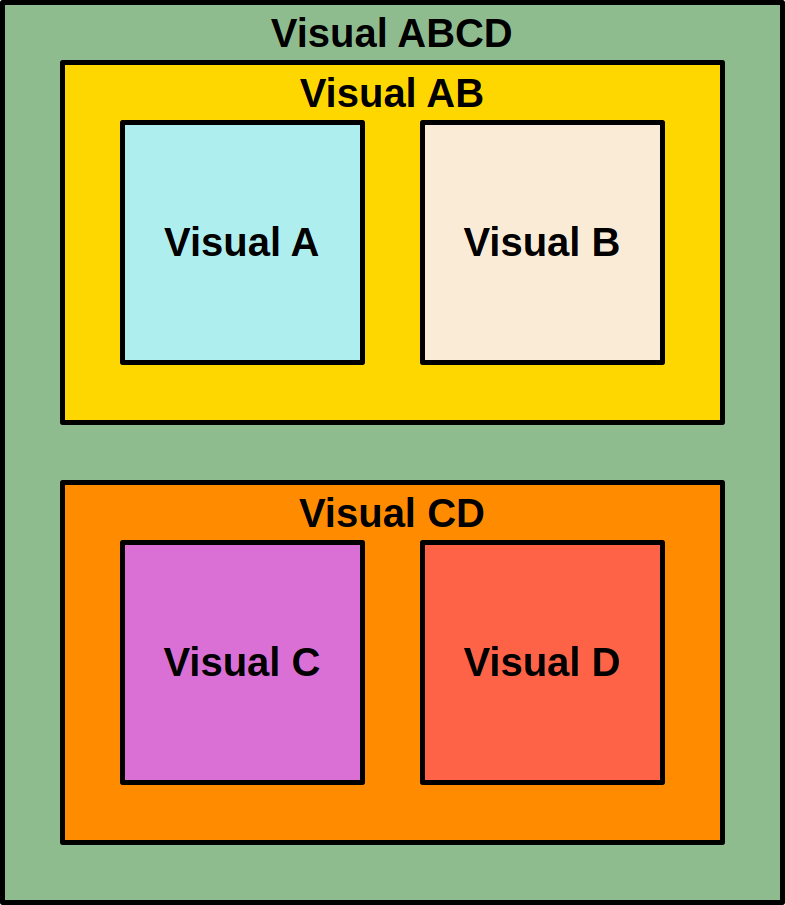
\includegraphics[width=0.4\textwidth]{figures/BlockDiagrams/LayersOnLayers.png}
  \caption{Composition of the LayerIt visualisation system. Each coloured box represents a distinct visual element that composes a higher-level visualisation.}
  \label{fig:LayersWithinLayers}
\end{figure}

This ``layers within layers'' design is applied at three levels of the project: the \textbf{visual level}, where visualisations combine aligned data, audio, and musical elements; the \textbf{SVG level}, where LayerIt organizes the XML structure of the output; and the \textbf{code level}, where the OO architecture organizes the corresponding program components. Together, these levels describe how individual elements are combined into composite visualisations.

\subsection{Visual Level}
At the visual level, layers are output elements aligned to a shared timeline. They can be arranged vertically in a composite view while retaining the temporal correspondence between the score, audio-derived representations, annotations, and BT output.

The concrete layer implementations are built on four shape abstractions. Each shape inherits from \texttt{Layer} and supplies the rendering behaviour for a particular kind of data; a concrete layer provides the data through the corresponding hook and configures its visual properties. The four shapes are:

\begin{itemize}
  \item \texttt{Curve}: represents a sampled two-dimensional signal as a line. It is suitable for continuous time-series data such as waveforms, activation curves, and onset-strength envelopes. A curve can use the panel's primary axis or a shared secondary axis.
  \item \texttt{Events}: represents a set of instantaneous time positions as vertical markers. It is used for discrete events such as onsets, beats, and downbeats.
  \item \texttt{Intervals}: represents contiguous regions selected from an activation signal after applying a threshold. These regions are rendered as highlighted windows, making periods of elevated activation visible across a panel.
  \item \texttt{Field}: represents a dense two-dimensional matrix, such as a time-frequency or time-pitch representation. The matrix is normalized and rendered as an embedded raster image, while its axes are added to the SVG group.
\end{itemize}

These abstractions separate the representation of data from the common rendering and SVG-export mechanisms. They are therefore the basis for implementing different layer types without requiring each layer to reimplement the complete drawing pipeline. The distinction also clarifies the intended visual encoding: curves show values over time, events show isolated time positions, intervals show selected time regions, and fields show values distributed over two dimensions.

\subsection{SVG Level}
At the SVG level, LayerIt organizes the XML structure of the output so that individual and combined layers remain identifiable. The following listing shows a simplified representation of the XML structure produced for a composed SVG file:

\pagebreak

\begin{lstlisting}[caption={Example structure of an SVG file},label={lst:svg-example}]
<svg>
|   <Top Visualisation>
|   |   <Layers>
|   |   |   <image spectrogram.png>
|   |   |   <BeatThis Output>
|   |   |   <Onsets>
|   |   <Score>
|   |   <timeAxis>
|   <Bottom Visualisation>
|   |   <Layers>
|   |   |   <Waveform>
|   |   |   <Beat Probability>
|   |   |   <Downbeat Probability>
</svg>
\end{lstlisting}

This XML organisation allows the SVG to be inspected and modified directly through its markup. It also preserves an identifiable structure for code-based processing while keeping the SVG readable. The nesting of elements at the XML level mirrors the visual composition described above.

\subsection{Code Level}

At the code level, LayerIt's OO architecture organizes each visualisation component as a self-contained module with a consistent interface. The same composition principle used at the visual and SVG levels is therefore represented in the code structure. The following snippets illustrate the base abstraction, the \texttt{Visualizer} composition API, and a short end-to-end workflow.

\begin{figure}[H]
  \centering
  
\includegraphics[width=\textwidth]{BlockDiagrams/Plot_ToSVG_to_SVGofSVG.png}
  \caption{TEMPORARY placeholder for the LayerIt architecture diagram. This figure reflects an earlier implementation.}
  \label{fig:architecture-placeholder}
\end{figure}

Listing \ref{lst:layer-base} shows an illustrative \texttt{Layer} base-class interface. The omitted imports are not relevant to the interface.

\pagebreak

\begin{lstlisting}[caption={Layer interface (concise)},label={lst:layer-base}]
class Layer(ABC):
  def __init__(self, name: str = "Layer"):
    self._data = None
    self.name = name

  @abstractmethod
  def load_data(self, **kwargs) -> bool:
    pass

  @abstractmethod
  def draw(self, ax: Axes, shared_data: Dict[str, Any]) \
           -> Tuple[List, List]:
    pass

  def to_svg_group(self, shared_data: Dict[str, Any]) \
                   -> Optional[str]:
    '''Optional SVG export for subclasses'''
    return None
\end{lstlisting}

In LayerIt, a \texttt{Visualizer} instance orchestrates the composition of multiple layers through a panel-based workflow. Layers are grouped into panels using \texttt{add\_panel()}, which allows multiple layers to be rendered together on the same axis. The \texttt{Visualizer} maintains a shared data dictionary that all layers access during rendering via \texttt{load\_all\_layers()} and \texttt{draw()}. The \texttt{compose()} method then renders all panels and combines them with the warped score into a final multi-panel SVG. Listing~\ref{lst:visualizer-api} shows the concise composition script used for the LBD figure.

\begin{lstlisting}[caption={Concise LayerIt composition script},label={lst:visualizer-api}]
fig = Visualizer(audio, score, maps, beats)
fig.add_panel(Onset(), BeatLogits(), DownbeatLogits(), height_scale=.5)
fig.add_panel(Waveform(), BeatsLayer(), DownbeatsLayer(), height_scale=.5)
fig.add_panel(MelSpec(freq_window=(100, 1500)))
fig.compose("LBD_FIG.svg")
\end{lstlisting}

The script initializes the shared inputs, groups layers into three panels, and delegates rendering and SVG assembly to \texttt{compose()}. The first two panels combine curves and event markers on shared axes, while the third adds a mel-spectrogram field. The lower-level panel rendering and SVG stacking operations are shown in Appendix~\ref{appendix:code-listings}.

LayerIt supports a workflow from matplotlib-based visualisation generation to SVG or PNG composition. The final composition stage can include externally produced graphics, allowing code-generated visualisations to be combined with images created outside the codebase.

This hybrid design supports multiple workflows, including Python-based prototyping and the use of externally generated images. Custom layer implementations and external image inputs can both be incorporated into the same composite visualisation.

These code-level choices provide the compositional mechanism validated in Chapter 5. The case study demonstrates that existing layers can be modified, exchanged, and regenerated through the common interface. The addition of entirely new layer types remains a direction for future work rather than a quantified result of this thesis.

\section{Summary}
This chapter closes the methodological and implementation stages of the thesis by connecting the development process described in Chapter 3 with the framework described in this chapter. The iterative path taken through the five prototypes clarified the scope of the work, showing that the most meaningful contribution was not a new annotation system, but a reusable visualisation framework grounded in time-aligned music data.

LayerIt was then shaped to answer that need: a Python OO framework for composing score-aligned MIR visualisations through layered SVG-based output. Its design emphasizes reuse, composability, and visual consistency, while relying on ScoreWarp for the alignment backbone and on established MIR libraries for the generation of the underlying audio and data layers. Taken together, the two chapters show how the project moved from exploratory prototyping to a focused implementation that can now be assessed against the criteria established in the methodology chapter.
